\begin{frame}{Однородная цепочка спинов}
  \begin{columns}
    \column{0.35\textwidth}
    \begin{figure}
      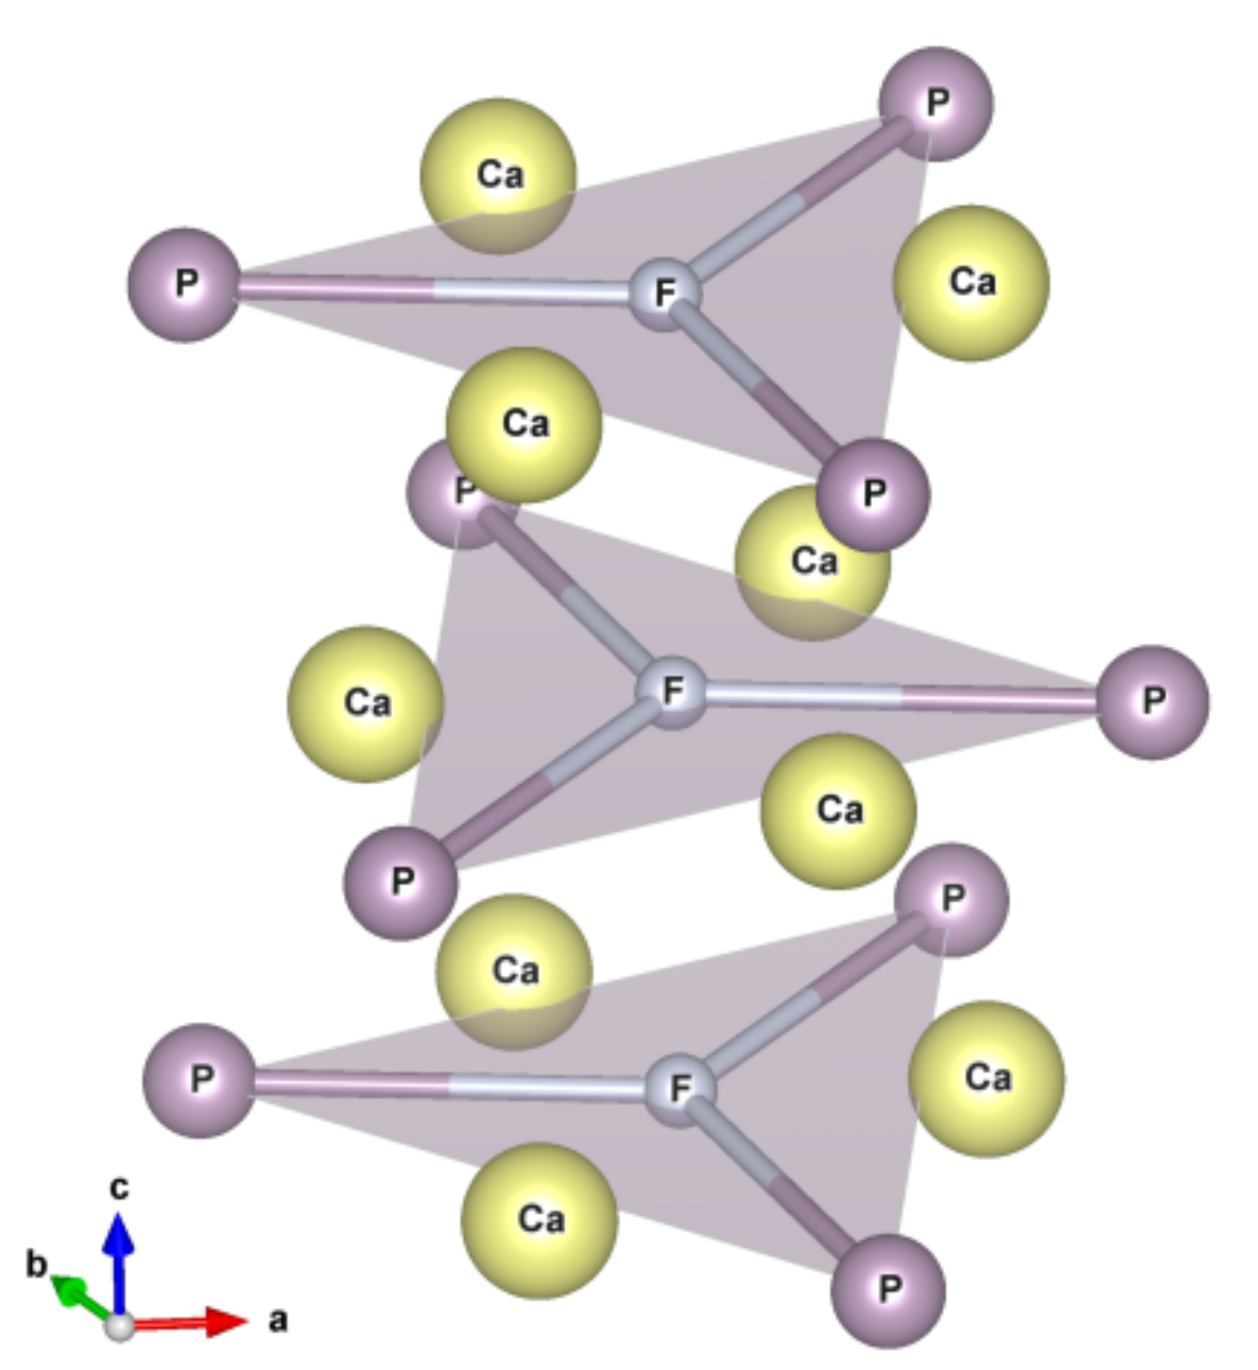
\includegraphics[width=\textwidth]{sample-fap-crystal-structure-part.png}
      \caption{Фтористый апатит Ca$_{10}$(PO$_4$)$_6$F$_2$}
    \end{figure}

    \column{0.6\textwidth}
      Часть кристаллической структуры FAp, показывающая окружение атомов фтора.
      Атомы кислорода были удалены для ясности.
      Атомы фтора равномерно разнесены ($r_{FF}= 3.44$\AA) и расположены в колонны вдоль $c$-оси кристалла.
      Каждый атом фтора окружен тремя равноудаленными атомами фосфора при $r_{FP} = 3.67$\AA,
      которые расположены в вершинах равносторонних треугольников на плоскости, перпендикулярной к $c$-оси,
      а также тремя ионами Ca\textrm{II} на расстоянии $2.34$\AA.
  \end{columns}
\end{frame}
\note{
  Фтористый апатит.
}
